\documentclass{standalone}
\usepackage{tikz}

\usetikzlibrary{math}

\begin{document}
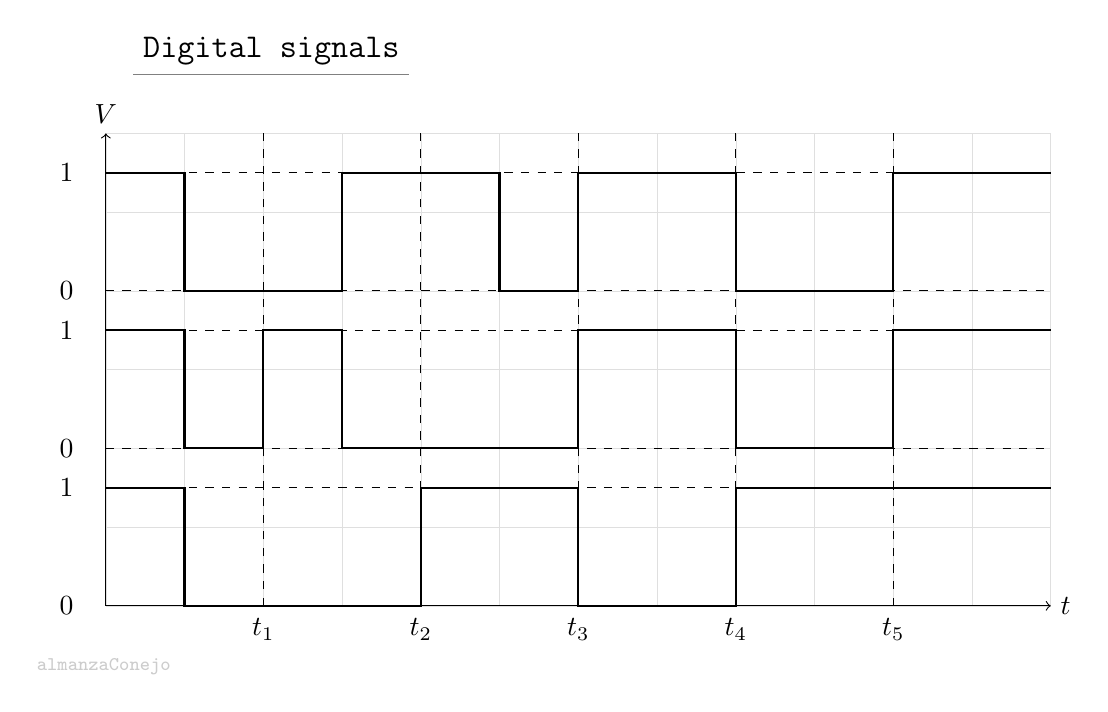
\begin{tikzpicture}
    \tikzmath{
        \ini1 = 0;
        \fin1 = 1.5;
        \ini2 = 2;
        \fin2 = 3.5;
        \ini3 = 4;
        \fin3 = 5.5;
        \xval = 12;
		\yval = 6;
    }

% líneas guía
\draw[help lines, gray!25]       (0, 0)  grid (\xval, \yval);

%title
%	--	title
\node[anchor = south west,
        font = \large] (title) at (0.35, \yval+0.75) {\texttt{Digital signals}};
\draw[gray] (title.south west) -- (title.south east);

% Ejes
\draw[->] (0,0) -- (\xval,0) node[right] {$t$};
\draw[->] (0,0) -- (0,\yval) node[above] {$V$};

% Líneas horizontales para cada señal con más espacio
\foreach \y in {0, 1.5, 2, 3.5, 4, 5.5} {
    \draw[dashed] (0,\y) -- (12,\y);
}

% Señales
% Primera señal
\draw[thick] (0,\fin3) -- (1,\fin3) -- (1,\ini3) -- (3,\ini3) -- 
                (3,\fin3) -- (5,\fin3) -- (5,\ini3) -- (6,\ini3) -- 
                (6,\fin3) -- (8,\fin3) -- (8,\ini3) -- (10,\ini3) -- 
                (10,\fin3) -- (12,\fin3);

% Segunda señal
\draw[thick] (0,\fin2) -- (1,\fin2) -- (1,\ini2) -- (2,\ini2) -- 
                (2,\fin2) -- (3,\fin2) -- (3,\ini2) -- (5,\ini2) -- 
                (5,\ini2) -- (6,\ini2) -- (6,\fin2) -- (8,\fin2) -- 
                (8,\ini2) -- (10,\ini2) -- (10,\fin2) -- (12,\fin2);

% Tercera señal
\draw[thick] (0,\fin1) -- (1,\fin1) -- (1,\ini1) -- (4,\ini1) -- 
                (4,\fin1) -- (6,\fin1) -- (6,\ini1) -- (8,\ini1) -- 
                (8,\fin1) -- (12,\fin1);

% Cuarta señal
%\draw[thick] (0,1) -- (1,1) -- (1,0) -- (2,0) -- (2,1) -- (3,1) -- (3,0) -- (4,0) -- (4,1) -- (6,1) -- (6,0) -- (7,0) -- (7,1) -- (9,1) -- (9,0) -- (10,0) -- (10,1) -- (12,1);

% Etiquetas de tiempo con t_5
\foreach \x/\t in {1/{$t_1$}, 2/{$t_2$}, 3/{$t_3$}, 4/{$t_4$}, 5/{$t_5$}} {
    \draw[dashed] (\x*2,0) -- (\x*2,6);
    \node at (\x*2,-0.3) {\t};
}

% Etiquetas de valores binarios con mejor posición

\node at (-0.5,\fin1) {1};
\node at (-0.5,\ini1) {0};
\node at (-0.5,\fin2) {1};
\node at (-0.5,\ini2) {0};
\node at (-0.5,\fin3) {1};
\node at (-0.5,\ini3) {0};

\node[%
		anchor = south west,
		text = gray!40,
		fill = white,
		align = left,
		font = \scriptsize,
	] (user) at (-1, -1) {\texttt{almanzaConejo}};

% \node[inner sep=0pt,
% 		fill = white,
% 		opacity = 0.40,
% 		anchor = north east] (ugto) at (\xval-0.1, \yval+1.25)
%     	{\includegraphics[width = 0.2\textwidth]{escudo-linea-horizontal-png.png}};

\end{tikzpicture}
\end{document}
